\documentclass[aspectratio=169,
				xcolor=table]{beamer}

% Load general definitions
\usepackage[utf8]{inputenc}
%\usepackage[T1]{fontenc}
\usepackage[brazil]{babel}
\usepackage{amsmath}
\usepackage{amsfonts}
\usepackage{amssymb}
\usepackage{graphicx}
\usepackage{verbatim}
\usepackage{cancel}
\usepackage{askmaps}
\usepackage{tabularx}
\usepackage[table]{xcolor}
%\usepackage{tikz}
\usepackage{multirow}
\usepackage{mathtools}
\usepackage{color, colortbl}
\usepackage{etoolbox}
\usepackage{pbox}
\usepackage{changepage}
\usepackage{xpatch}
\usepackage{array}
\usepackage{marvosym}
\usepackage{tabu}
\usepackage{multicol}
\usepackage{listings}
\usepackage{underscore}
\usepackage{filecontents}
\usepackage[]{algorithm2e}
\usepackage{ragged2e}

\newcolumntype{P}[1]{>{\centering\arraybackslash}m{#1}}
\definecolor{Gray}{gray}{0.75}
\definecolor{Gray2}{gray}{0.85}

\definecolor{lightBlue}{HTML}{DAE8FC}
\definecolor{Blue}{RGB}{51, 51, 204}

%\useinnertheme[lily]{rounded}
\usetheme{UniEvangelica}
%\usetheme{Copenhagen}
%\usetheme{Berlin}
%\usecolortheme{dolphin}
\tolerance=1
\emergencystretch=\maxdimen
\hyphenpenalty=10000
\hbadness=10000

\setbeamertemplate{navigation symbols}{}%remove navigation symbols


\let\olditem=\item% 
\renewcommand{\item}{\olditem \justifying}%
\def\center{\trivlist \centering\item\relax}
\def\endcenter{\endtrivlist}

\setbeamertemplate{itemize/enumerate body begin}{\large}
\setbeamertemplate{itemize/enumerate subbody begin}{\large}

\setbeamertemplate{itemize item}{\raisebox{0.1ex}{$\blacktriangleright$}\hskip0.1em}
\setbeamertemplate{itemize subitem}{\raisebox{0.1ex}{$\blacktriangleright$}\hskip0.1em}

\newcommand{\greenarrow}{\textcolor{green}{\rotatebox[origin=c]{180}{\MVArrowDown}}}

\newcommand{\redarrow}{\textcolor{red}{\MVArrowDown}}

%\newcommand{\ftable}{
%	\begin{table}
%		\large
%		\centering
%		\rowcolors{1}{\ifnumless{\rownum}{2}{Blue}{lightBlue}}{}
%}

\newenvironment{eftable}{
	\begin{table}
		\large
		\centering
		\rowcolors{1}{}{Blue}
		\rowcolors{1}{\ifnumless{\rownum}{2}{Blue}{lightBlue}}{}
	}
	{
	\end{table}
}


%\setbeamertemplate{frametitle}
%{
%	%\vspace*{-2em}	
%	\insertframetitle
%
%	 %\textcolor{white}{\LARGE \insertframetitle}
%
%}

% Specific definitions
\institute[]{\uppercase{Engenharia de Software}}
\title[]{Sistemas Operacionais}
\subtitle[]{Threads}
\author[]{Prof. M.e Alexandre Tannus}
\date{Anápolis - 2021.1}

%\AtBeginSection{\frame{\tableofcontents[currentsection]}}

\begin{document}
	\begin{frame}
		\titlepage
	\end{frame}

	\begin{frame}
		\tableofcontents
	\end{frame}	
	
	\section{Introdução}
	
	\begin{frame}{Questionamentos}
		\begin{itemize}
			\item Como implementar concorrência dentro de uma aplicação?
			\vspace{1em}
			\item O que é uma \textit{thread}?
			\vspace{1em}
			\item Quais são os modelos de configuração de uma \textit{thread}?
			\vspace{1em}
			\item Existem problemas em trabalhar com sistemas \textit{multithread}?
		\end{itemize}
	\end{frame}

	\section{Introdução}
	\begin{frame}{Relembrando...}
		\alert{\Large Definição}
		\begin{itemize}
			\item Programa
			\begin{itemize}
				\item Conjunto de instruções para realizar uma tarefa
				\item Entidade passiva
			\end{itemize}
			\vspace{1em}
			\item Processo
			\begin{itemize}
				\item Entidade ativa
				\item Contém informações sobre a execução
			\end{itemize}
		\end{itemize}
	\end{frame}
	
	\begin{frame}{Relembrando...}	
		\alert{\Large Estrutura do Processo}
		\begin{figure}[hbtp]
			\centering
			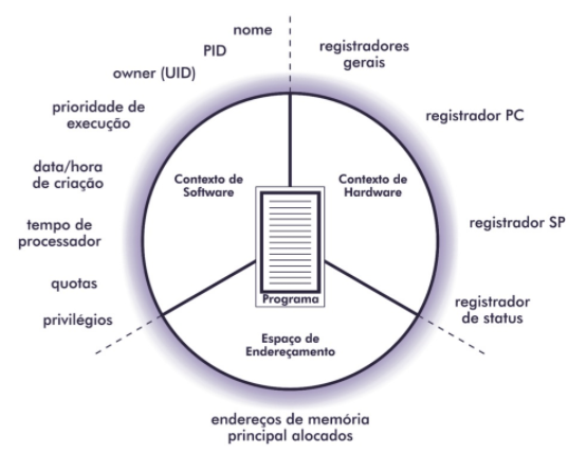
\includegraphics[keepaspectratio, height=.7\textheight]{../figs/cap04/estrutura1.png}
		\end{figure}
	\end{frame}
	
	\begin{frame}{Relembrando...}
		\alert{\Large Bloco de Controle do Processo - BCP}
		\vspace{1em}
		\begin{itemize}
			\item Estrutura de dados responsável pela implementação do processo pelo sistema operacional
			\vspace{1em}
			\item Mantém informações sobre o contexto de hardware, contexto de software e espaço de endereçamento de cada processo
			\vspace{1em}
			\item Armazenados em área exclusiva na memória principal
			\begin{itemize}
				\item Tamanho da área pode ser configurado no sistema operacional
			\end{itemize}
		\end{itemize}
	\end{frame}
	
	\begin{frame}{Concorrência}
		\begin{itemize}
			\item Subdivisão do código em partes para trabalhar de forma cooperativa
			\vspace{1em}
			\item Formas
			\begin{itemize}
				\item Processos independentes
				\item Subprocessos
				\item \textit{Threads}
			\end{itemize}
		\end{itemize}		
	\end{frame}
	
	\begin{frame}{Processos independentes}
		\begin{itemize}
			\item Forma mais simples
			\vspace{1em}
			\item Sem vínculo entre o processo criado e o processo criador
			\begin{itemize}
				\item Alocação de PCB exclusivo para o novo processo
			\end{itemize}
		\end{itemize}		
	\end{frame}
	
	\begin{frame}{Subprocessos}
		\begin{itemize}
			\item Estrutura hierárquica
			\begin{itemize}
				\item \textbf{Processo criador}: processo-pai
				\item \textbf{Subprocesso}: processo-filho
			\end{itemize}
			\vspace{1em}
			\item Possibilidade de criação de novos processos por um processo-filho
			\vspace{1em}
			\item Cada subprocesso possui um PCB próprio
			\begin{itemize}
				\item Possibilidade de compartilhamento de quotas
			\end{itemize}
		\end{itemize}		
	\end{frame}
	
	\begin{frame}{Subprocessos}		
		\begin{figure}[hbtp]
			\centering
			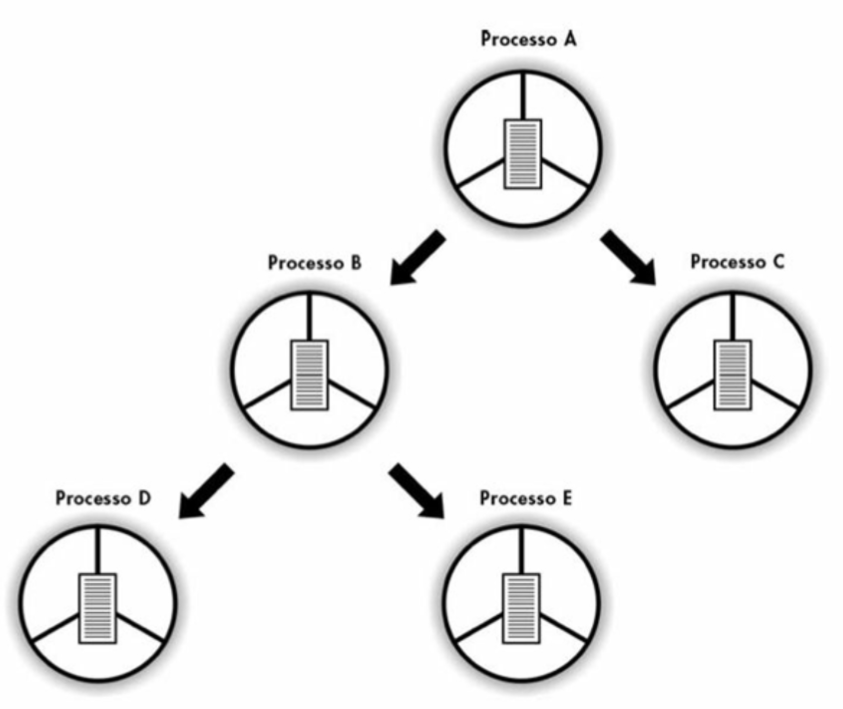
\includegraphics[keepaspectratio, height=.8\textheight]{../figs/cap04/subprocessos.png}
		\end{figure}
	\end{frame}
	
	\begin{frame}{Criação de processos - Desvantagens}
		\begin{itemize}
			\item Consumo de recursos do sistema
			\begin{itemize}
				\item BCP próprio (contexto de hardware, contexto de software e espaço de endereçamento)
				\item Tempo de CPU (alocação e desalocação)
			\end{itemize}
			\vspace{1em}
			\item Comunicação e sincronização entre processos ineficiente
		\end{itemize}		
	\end{frame}
	
	\section{\textit{Threads}}
	
	\begin{frame}{Threads - Definição}
		\begin{itemize}
			\item Unidade básica de utilização da CPU
			\vspace{1em}
			
			\begin{figure}[hbtp]
				\centering
				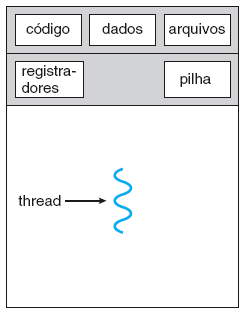
\includegraphics[keepaspectratio, height=.6\textheight]{../figs/cap04/monothread.png}
			\end{figure}
		\end{itemize}
	\end{frame}
	
	\begin{frame}{Threads - Características}
	
		\begin{columns}[t]
			\begin{column}{0.5\textwidth}			
				\begin{itemize}
					\item Contexto de hardware exclusivo para cada \textit{thread}
					\vspace{1em}
					\item Compartilhamento de contexto de software e espaço de endereçamento em \textit{threads} do mesmo processo					
				\end{itemize}
			\end{column}
			\begin{column}{0.5\textwidth}
			\begin{figure}[hbtp]
				\centering
				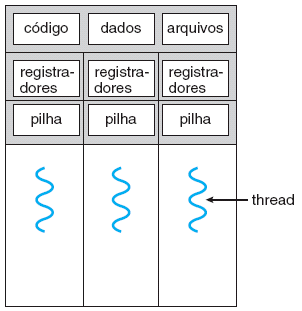
\includegraphics[width=.85\textwidth, keepaspectratio]{../figs/cap04/multithread.png}
			\end{figure}
			\end{column}
		\end{columns}
	\end{frame}

	\begin{frame}{Ambiente multithread}
		\begin{figure}[hbtp]
			\centering
			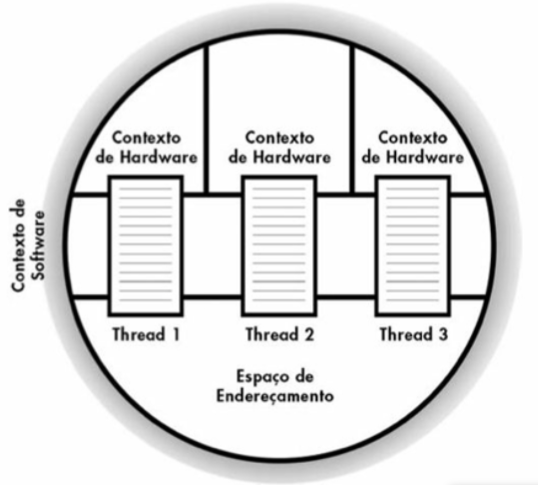
\includegraphics[height=.85\textheight, keepaspectratio]{../figs/cap04/multithread02.png}
		\end{figure}	
	\end{frame}	
	
	\begin{frame}{Benefícios}
		\begin{itemize}
			\item Capacidade de resposta
			\vspace{1em}
			\item Compartilhamento de recursos
			\vspace{1em}
			\item Economia
			\vspace{1em}
			\item Escalabilidade
		\end{itemize}
	\end{frame}
	
	\section{Modelos de Multithreads}
	
	\begin{frame}{Modelos de Multithreads}
		\begin{itemize}
			\item Suporte aos \textit{threads} em nível de usuário ou kernel
			\vspace{1em}
			\item Nível usuário
			\begin{itemize}
				\item Suportados acima do kernel 
				\item Gerenciados sem o suporte do kernel
			\end{itemize}
			\vspace{1em}
			\item Nível kernel
			\begin{itemize}
				\item Suportados e  gerenciados pelo sistema operacional
			\end{itemize}
		\end{itemize}
	\end{frame}
	
	\begin{frame}{Threads nível usuário}
		\begin{itemize}
			\item Vantagens
			\begin{itemize}
				\item Troca de contexto sem necessidade do kernel
				\item Escalonamento baseado na aplicação
				\item Programa pode rodar em qualquer sistema operacional
			\end{itemize}
			\vspace{1em}
			\item Desvantagens
			\begin{itemize}
				\item Bloqueio de todos os \textit{threads} do processo em caso de chamada ao sistema (\textit{system call})
				\item Processo completo é designado a um processador
			\end{itemize}
		\end{itemize}
		
	\end{frame}
	
	\begin{frame}{Threads nível kernel}
		\begin{itemize}
			\item Vantagens
			\begin{itemize}
				\item Bloqueio em nível de thread
				\item Kernel pode designar threads para qualquer processador
				\item Rotina do kernel pode ser \textit{multithreaded}
			\end{itemize}
			\vspace{1em}
			\item Desvantagens
			\begin{itemize}
				\item Troca de threads exige mudança para modo kernel
			\end{itemize}
		\end{itemize}
	\end{frame}
	
	\begin{frame}{Relacionamento entre threads usuário-kernel}

		\begin{figure}[hbtp]
			\centering
			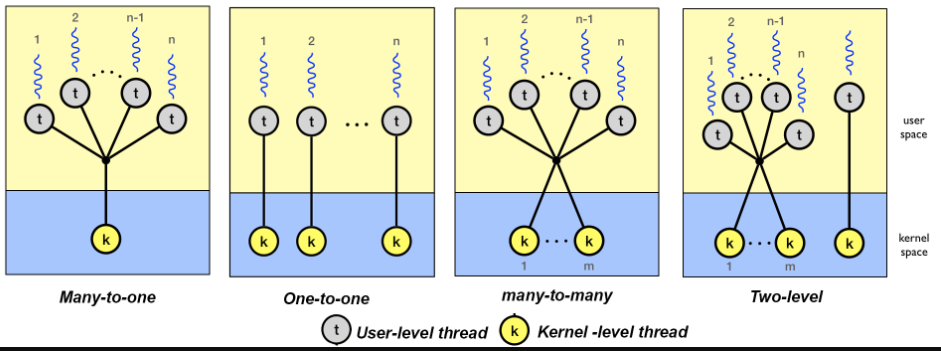
\includegraphics[width=.85\textwidth, keepaspectratio]{../figs/cap04/threadrelation.png}
		\end{figure}		
	\end{frame}
	
	\begin{frame}{Bibliotecas de Threads}
		\begin{itemize}
			\item API (\textit{Application Programming Inteface}) para criação e gerenciamento de threads
			\item Principais bibliotecas
			\begin{itemize}
				\item Pthreads (POSIX)- usuário ou kernel
				\item Windows - kernel
				\item Java - dependente do sistema hospedeiro
			\end{itemize}
		\end{itemize}
	\end{frame}
	
	\begin{frame}{Detalhes da programação}
		\begin{itemize}
			\item Dados declarados globalmente e compartilhados por todos os \textit{threads} do mesmo processo (POSIX e Windows)
			\item Formas de criação de \textit{threads}
			\begin{itemize}
				\item Assíncrona (execução concorrente de pai e filho)
				\item Síncrona (pai deve esperar finalização da execução dos filhos)
			\end{itemize}			
		\end{itemize}		
	\end{frame}
	
	\begin{frame}{Problemas com threads}
		\begin{itemize}
			\item Efeitos da chamada de sistema \textit{fork}
			\item Compartilhamento de estrutura de dados
			\item Informe de erros
			\item Gerenciamento de sinais
			\item Gerenciamento da pilha
		\end{itemize}
		
	\end{frame}
	
	\begin{frame}{Bibliografia}
		\begin{itemize}
			\item SILBERSCHATZ, A.; GALVIN, P. B.; GAGNE, G.. \textbf{Fundamentos de sistemas operacionais: princípios básicos.} Rio de Janeiro: LTC – Livros Técnicos e Científicos, 2013.
			
			\vspace{1em}

			\item TANENBAUM, A.S., WOODHULL, A.S. \textbf{Sistemas Operacionais.} Porto Alegre: Grupo A, 2008.
			
			\vspace{1em}
			
			\item MACHADO, F.B.; MAIA, L.P. \textbf{Fundamentos de Sistemas Operacionais.} Porto Alegre: Grupo GEN, 2011.
		\end{itemize}
	\end{frame}


	\begin{frame}{}
	\end{frame}	
	
\end{document}
